\documentclass[12pt]{article}

\usepackage[letterpaper, hmargin=0.75in, vmargin=0.75in]{geometry}
\usepackage{float}
\usepackage{url}
\usepackage{graphicx}
\graphicspath{ {./images/} }

\pagestyle{empty}

\title{ECE 459: Programming for Performance\\Assignment 4}
\author{Zhidong Zhang}
\date{March 31, 2020}

\begin{document}

\maketitle
\section*{1: Analyze the slow Flamegraph}
This is the initial Flamegraph of the slow version:\\
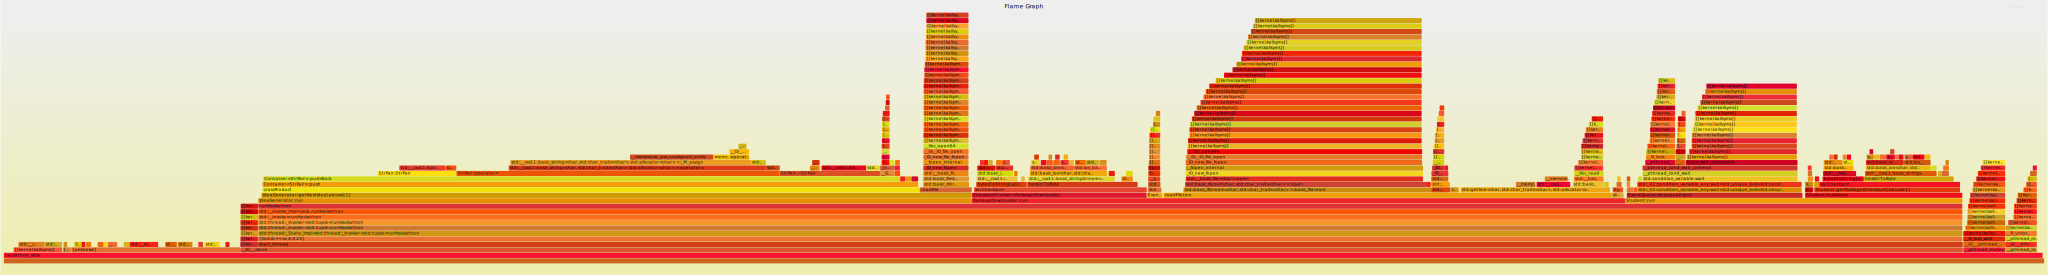
\includegraphics[width=1\columnwidth]{images/perf_slow.png}\\
We can identify which functions or procedures are taking a long time, and we can optimize from there. According to the initial Flamegraph of the slow version, three functions take up the majority of the execution time. The first one is $Container<StrPair>::pushBack$, which took 31.21\%. The second one is $readFileLine$, which took 21.96\%. The third one is $xorChecksum$, which took 15.77\%. I focused on those three functions and optimized them.
\section*{2: My Changes}
\begin{enumerate}
\item Container:
   \begin{itemize}
     \item After investigating the code in the Container.h, I found out that it uses a fix size array as the data structure for storage. The fix size array makes pushFront, pushBack, popFront have O(n) time complexity, which is slow. I changed the fix size array to \textbf{deque}, which is a double-ended queue. Deque supports O(1) pushFront, O(1) pushBack, and O(1) popFront. After changing the fix size array to deque, the program gets a 2x speedup.
   \end{itemize}
\item readFileLine + PackageDownloader::run:
   \begin{itemize}
     \item After investigating the readFileLine function, I found out that, to get a line by line number, it starts from the beginning of the file every single time, which means O(n) time complexity. In function PackageDownloader::run, calling the readFileLine by n times is O($n^2$) time complexity, which is slow. To reduce the time complexity, I made some changes in function PackageDownloader::run. First, I use the readFile function to read the "data/packages.txt" into a container named as packages, which support O(1) index access. Then, for each package index i, I just use \textbf{packages[i \% packages.size()];} to get the package name. The reason I use mod operation is that the package index i can be greater than the package size, so we need to read from the start of the packages again. By making this change, the time complexity for getting the package name by index has been reduced from O(n) to O(1), and the program shows significant speedup. 
   \end{itemize}
\item xorChecksum:
   \begin{itemize}
     \item After investigating the xorChecksum function, I found out that it first convert the hex string to byte, do the XOR operation, then convert the XOR result back to hex string. There is lots of redundant work. We can use the uint8\_t* type to represent the checksum, and then we can do the XOR operation directly. Therefore, I changed every checksum from string type to uint8\_t* type, and also change the return type of xorChecksum function, sha256 function and initChecksum function to uint8\_t*. After this change, the program shows significant speedup.
   \end{itemize}
\end{enumerate}
\section*{3: Final Result (Flamegraph + Speedup)}
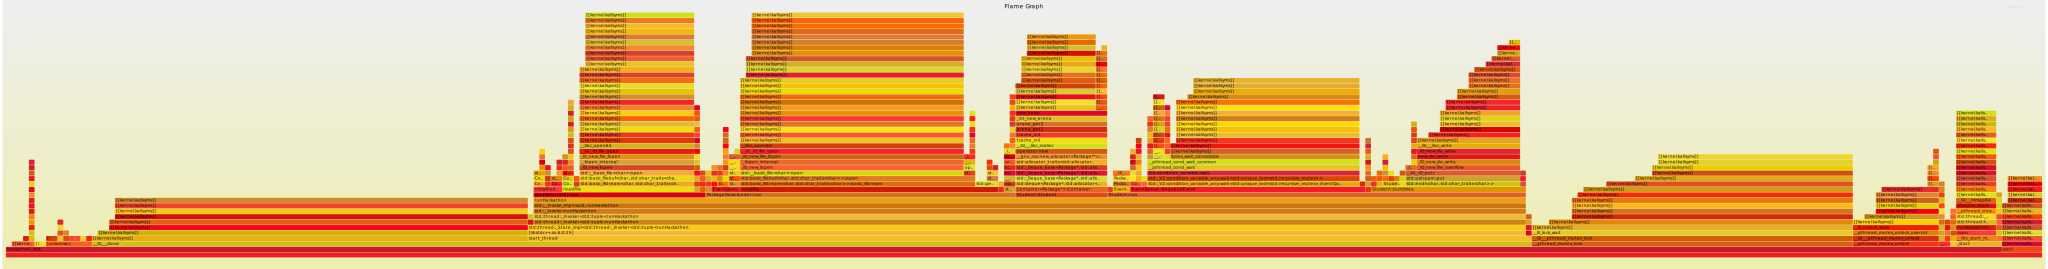
\includegraphics[width=1\columnwidth]{images/perf_fast.png}
\\
\\
$\begin{array}{ | l | l | l | l | l | }
\hline
	 & run\_slow & run\_fast \\ \hline
	Run\:1 & 1.821\:s & 0.0398\:s \\ \hline
	Run\:2 & 1.876\:s & 0.0396\:s \\ \hline
	Run\:3 & 1.887\:s & 0.0391\:s \\ \hline
	Run\:4 & 1.877\:s & 0.0395\:s \\ \hline
	Average & 1.865\:s & 0.0395\:s \\ \hline
	Speed up & & 47\:times \\ \hline
\end{array}$ \\
\\
\\
From the final Flamegraph, we can see that $Container<StrPair>::pushBack$ only takes 0.56\% of the total execution time, $PackageDownloader::run$ takes 15\% of the total time, and $xorChecksum$ only takes 0.28\%. All three slow functions are optimized successfully. The total execution time was reduced from 1.865 s to 0.0395 s, which is 47 times speedup.
\end{document}
